\chapter{Implementierung und Benchmarks}

In diesem Kapitel wird die Implementierung der in Kapitel 3 eingeführten Algorithmen zur Berechnung der QR-Zerlegung mittels Householder-Transformation beschrieben. 
Die verwendete Bibliothek, der Fehlerschätzer und die Benchmarks werden erläutert. 

Die verwendete Bibliothek wurde in der Vorlesung High Performance Computing 1 entwickelt \cite{HPC1} und wird im folgenden HPC1-Bibliothek genannt.


Die Implementierung steht auf GitHub Verfügung \cite{git}.\\
Link: \url{https://github.com/Flousen/Bachelorarbeit}

\section{Bibliothek}
Die HPC1-Bibliothek ist in C++ geschrieben und stellt eine Schnittstelle zu den BLAS-Routinen der IntelMKL zur Verfügung.
Das ermöglicht, die Algorithmen mit den BLAS-Routinen zu implementieren.
Dabei wurde sich an der Implementierung LAPACK orientiert.


Die HPC1-Bibliothek enthält Klassen für Matrizen und Vektoren.
Die Matrix-Klassen erlauben den Zugriff auf Matrixblöcke. 
Der folgende Code soll beispielhaft den Zugriff auf Matrixblöcke veranschaulichen.
\begin{lstlisting}
GenerelMatrix<T> A(5,5);  // erzeugt Matrix-Objekt
init(A);  // Matrix mit Zufallszahlen initialisieren
printf("A   =\n");print(A); // Matrix ausgeben
printf("A22 =\n");print(A.block(2,2));
printf("A22T=\n");print(A.block(2,2).view(Trans::view));
\end{lstlisting}
Der Code erzeugt erzeugt zuerst eine $5 \times 5$ Matrix.
Die Funktion \textit{init} initialisiert die Matrix zeilenweise mit den Werten 1 bis 25.
Diese Matrix wird 3 ausgegeben. Zuerst die komplette Matrix(Zeile 3), dann eine ein Block der Matrix beginnend in der dritten Zeile und dritten Spalte. Als letztes wird der selbe Matrix Block noch Transponiert betrachtet.Der Code kann die folgende Ausgabe erzeugen.
\lstset{numbers=none}
\begin{lstlisting} 
A   = 
      1    2    3    4    5
      6    7    8    9   10
     11   12   13   14   15
     16   17   18   19   20
     21   22   23   24   25

A22 = 
     13   14   15
     18   19   20
     23   24   25

A22T= 
     13   18   23
     14   19   24
     15   20   25
\end{lstlisting}

\subsubsection{MKL Wrapper}
Um von der Bibliothek auf Blas-Routienen der MKL zugreifen zu können, benötigt man Wrapper, die die Schnittstelle zur MKL darstellen.

MKL-Blas-Routinen kennen keine Matrix- und Vektor-Klassen, wie es sie in der HPC1-Bibliothek gibt. Diese Funktionen bekommen Zeiger auf die Daten und Verwaltungsinfomationen als Variable übergeben.
Die Wrapper extrahieren die Daten aus den Klassen und rufen damit die MKL-Funktionen auf.

Der folgende Code zeigt einen solchen Wrapper am Beispiel der Skalarprodukt-Funktion \textit{dot}.
\lstset{numbers=left,firstnumber=14}
\begin{lstlisting}
double
dot(MKL_INT n, const double *x, MKL_INT incx,
    const double *y, MKL_INT incy)
{
  return ddot(&n, x, &incx, y, &incy);
}

template <typename T, template<typename> class VectorX,
                      template<typename> class VectorY,
          Require< Dense<VectorX<T>>,
                   Dense<VectorY<T>> > = true>
T
dot(const VectorX<T> &x, const VectorY<T> &y)
{
  return dot(x.length(), x.data(), x.inc(), 
             y.data(), y.inc());
}
\end{lstlisting}
Die Funktion in den Zeilen 21--30 wird von der Bibliothek aufgerufen.
In den Zeilen 28 und 29 werden die für die Funkton wichtigen Parameter aus den Klassen ausgelesen und damit die Wrapper-Funktion (Zeilen 14--19) aufgerufen. Die Wrapper-Funktion ruft die Blas-Funktion auf (Zeile 18).


\subsection{Algorithmus}

Beispiel: Ungeblockte QR-Implementierung vom Algorithmus \ref{alg:unblockedqr} (Seite \pageref{alg:unblockedqr})
\lstset{numbers=left,firstnumber=1}
\begin{lstlisting}
size_t mn = std::min(m,n);
DenseVector<T> work(mn);
for (std::size_t i = 0; i < m
n; ++i){
  householderVector(A(i,i), A.col(i+1,i),tau(i));
  if (i < n && tau(i) != 0) {
    AII = A(i,i);
    A(i,i) = 1;
    mv(1, A.block(i,i+1).view(hpc::matvec::Trans::view),
       A.col(i,i), 0, work.block(i+1));
    rank1(-tau(i), A.col(i,i), work.block(i+1), 
          A.block(i,i+1));
    A(i,i) = AII;
  }
}
\end{lstlisting}

Die anderen Algorithmen wurden analog implementiert, siehe Anhang.

\section{Fehlerschätzer} \label{Fehlerschätzer}

Um zu testen, ob die QR-Zerlegung korrekt ist, ist ein Fehlerschätzer notwendig.
Es wurde der Fehlerschätzer von ATLAS \cite{atlas} verwendet.
\begin{align}
err = \dfrac{\|A - QR\|_i}{\|A\|_i \cdot \min(m,n) \cdot \varepsilon}
\end{align}
$\|\cdot\|_i$ ist eine passende Norm.
Die Matrizen $Q$ und $R$ sind die QR-Zerlegung der Matrix $A \in \mathbb{R}^{m \times n}$.
$\varepsilon$ ist die kleinste darstellbare Zahl.\\
Die QR-Zerlegung ist gut genug, falls der Fehler kleiner 1 ist: $ err < 1 $.

Als Norm wurde die Zeilensummennorm $\|\cdot\|_\infty$ gewählt.
Diese ist für eine Matrix $A \in \mathbb{R}^{m\times n}$ gegeben durch
\begin{align*}
\|A\|_\infty = \max_{i=1,...,m} \sum_{j=1}^{n} |a_{ij}|
\end{align*}

Diese Norm wurde gewählt, da sie für zeilenweise gespeicherte Matrizen effizient berechnet werden kann.

\section{Benchmarks}

\subsection{Aufwand} \label{aufwand}

Der Aufwand zur Berechnung der QR-Zerlegung mittels Householder-Transformation einer Matrix $A \in \mathbb{R}^{m \times n},~~ m \ge n$ ist bei ATLAS \cite{atlas} angegeben mit
\begin{align}
%\# &= n^2(m-\frac{1}{3} n) + {\cal O}(mn) \\
\#\text{QR} &= n \cdot \left(\frac{23}{6} + m + \dfrac{n}{2} + n\cdot \left(\frac{m-n}{3} \right) + n\cdot \left(\dfrac{5}{6} + \dfrac{n}{2} + m - \dfrac{n}{3}\right)\right) %= {\cal O}(n^2m)
\label{OQR}
\end{align}
$\#\text{QR}$ bezeichnet die Anzahl der Rechenoperationen, die zur Berechnung der QR-Zerlegung notwendig sind. 
Vereinfacht man (\ref{OQR}), dann erhält man einen Aufwand von $ {\cal O}(n^2m)$.

\subsection{FLOPS}
FLOPS (\textit{floating point operations per second}) geben an, wie viele Fließkomma-Operationen pro Sekunde ausgeführt werden.
\begin{align*}
  \text{FLOPS} = \dfrac{\#}{\Delta t}
\end{align*}
$\Delta t$ bezeichnet die Zeit in Sekunden und $\#$ die Anzahl der Rechenoperationen, die zur Berechnung benötigt werden.

\subsection{Vorgehensweise}

Ein $m \times n$ Matrix wird mit gleichverteilten Zufallswerten aus $[-1,1]$ initialisiert.

Die Matrix wird kopiert, um nach der Berechnung den Fehler schätzen zu können. Die QR-Zerlegung wird von der kopierten Matrix berechnet. Es wird die Zeit gemessen welche für die Berechnung benötigt wird. 
Aus der Originalmatrix und der kopierten QR-zerlegten Matrix wird der Fehler berechnet, so wie in Abschnitt \ref{Fehlerschätzer} beschrieben.

Aus den Matrix-Dimensionen wird die Anzahl der Rechenoperationen berechnet (Abschnitt \ref{aufwand}).
Aus Anzahl der notwendigen Rechenoperationen und der gemessenen Zeit werden die FLOPS berechnet.

Es wurden jeweils Matrizen mit den Dimensionen $10 \times 10$ bis $1000 \times 1000$  getestet. Die Matrizen wurden in Zehnerschritten vergrößert.


\subsection{Testsystem}

Getestet wurde auf einem System mit einer Intel i5-3470-CPU mit 3,20 GHz. 
Auf der Architektur dieses Prozessors errechnet sich die theoretische Maximalleistung (\textit{peak performance}) aus der Taktrate mal die Registerbreite mal 2. 

%Die theoretische Maximalleistung (\textit{peak performance}) errechnet sich, auf der Architektur des Prozessors, aus der Taktrate mal die Registerbreite mal 2. 

Die CPU des Testsystems hat eine Taktrate von 3,20 GHz.
Die AVX-Register haben eine Größe von 256 Bit.
%Die AVX-Register sind 256 Bit groß. 
Darin haben 4 \textit{double} Platz.
\begin{align*}
  \text{Taktrate} \cdot \text{Registerbreite} \cdot 2= 3,20 \text{ GHz} \cdot 4 \cdot 2 = 25,6 \text{ GFLOPS}
\end{align*}

\newpage
\section{Ergebnisse}
\subsection{Ungeblockter Algorithmus}
Die Abbildung \ref{img:unblk} zeigt den Vergleich des selbst implementierten Algorithmus \ref{alg:unblockedqr} (Seite \pageref{alg:unblockedqr}) mit dem ungeblockten Algorithmus der MKL (\textit{dgeqrf2}).

Ab einer Matrix-Dimension von $400 \times 400$ bleibt die Anzahl FLOPS gleichmäßig über 7 GFLOPS. Dieser Wert liegt weit unter 25,6 GFLOPS, der theoretischen \textit{peak performance}. 

%Mit dem Ungeblockten Algorithmus erreicht man die theoretische \textit{peak performance} 25 600 MFLOPS nicht. 



\begin{figure}[H]
	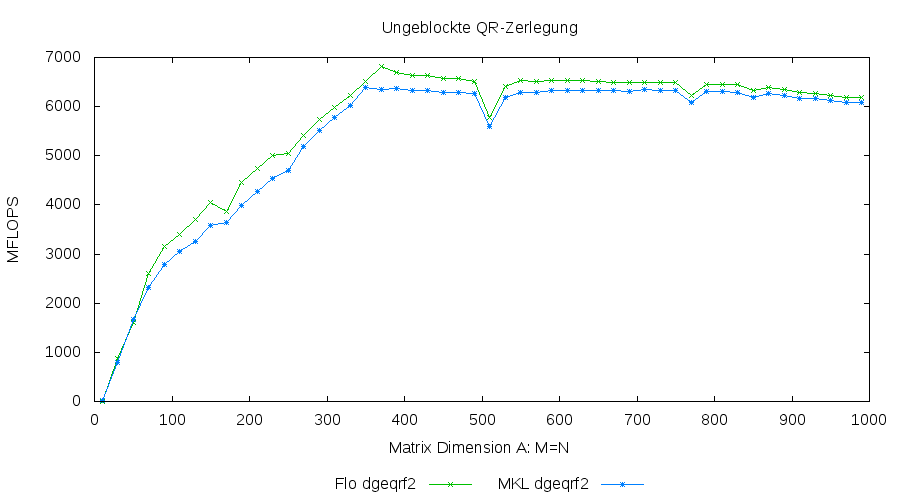
\includegraphics[width=\textwidth]{images/unblk.png}
	\caption{Benchmark ungeblockte QR-Zerlegung}
	\label{img:unblk}
\end{figure}



\subsection{Cache-optimierter Algorithmus}

Die Abbildung \ref{img:blkbs} zeigt den Vergleich des Algorithmus \ref{alg:blockedqr} (Seite \pageref{alg:blockedqr}) mit verschiedenen Blockgrößen.

Als Blockgrößen wurden die Zweierpotenzen $2^3 = 8$ bis $2^7 = 128$ getestet.


\begin{figure}[H]
	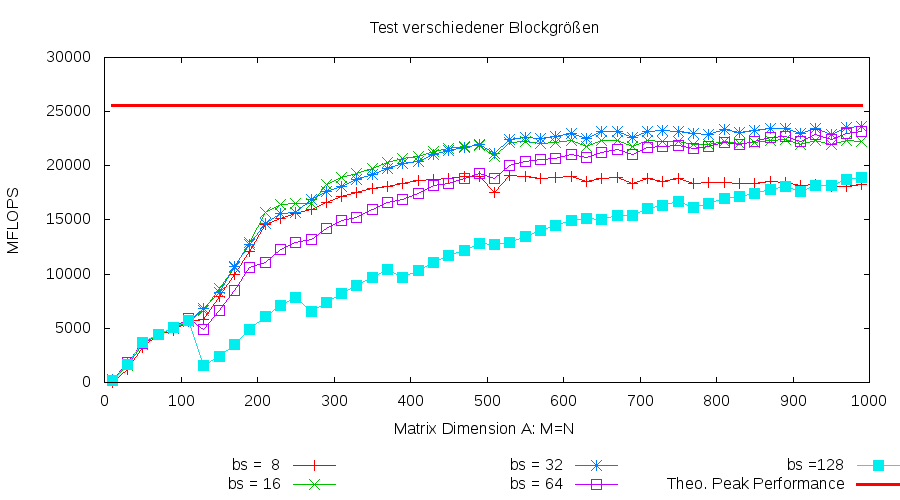
\includegraphics[width=\textwidth]{images/blkbs.png}
	\caption{Benchmark geblockte QR-Zerlegung}
	\label{img:blkbs}
\end{figure}
\newpage

Die Abbildung \ref{img:blk} zeigt den Vergleich des selbst implementierten Algorithmus \ref{alg:blockedqr}, mit Blockgröße $32$, mit dem Algorithmus  \textit{dgeqrf} aus der MKL.
\textit{dgeqrf} ist der cache-optimierte Algorithmus zur Berechnung der QR-Zerlegung.

Beide Implementierungen sind von der Performance sehr ähnlich und erreichen fast die \textit{peak performance}. Dabei ist die Implementierung der MKL etwas besser.

Zusätzlich sind in der Abbildung \ref{img:blk} noch die Benchmark-Ergebnisse der ungeblockten Algorithmen eingezeichnet. Hier wird der Performancegewinn des geblockten Algorithmus deutlich.

\begin{figure}[H]
  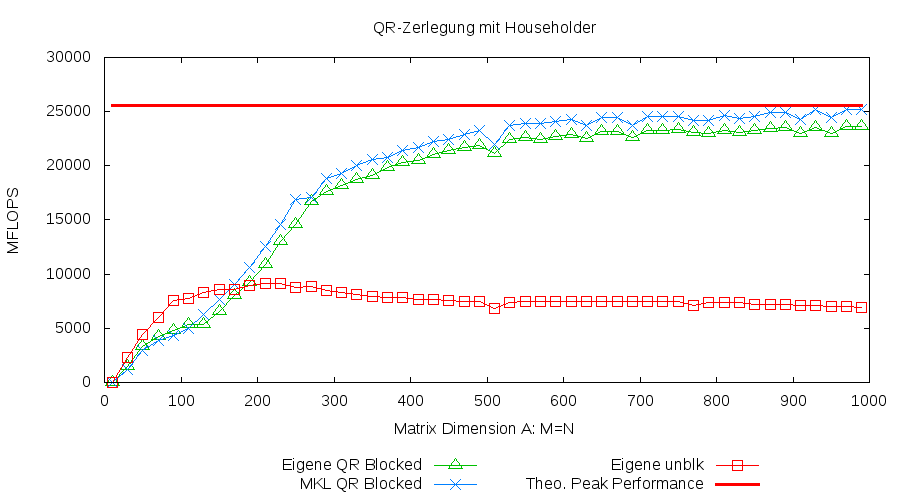
\includegraphics[width=\textwidth]{images/both.png}
  \caption{Benchmark geblockte QR-Zerlegung}
  \label{img:blk}
\end{figure}


\newpage
\section{Fazit}
Die Benchmarktests erbrachten die folgende Ergebnisse:
\begin{itemize}
	\item Der ungeblockte Algorithmus beider Implementierungen erreicht nicht die \textit{peak performance}.
	\item Der selbst programmierte ungeblockte Algorithmus ist etwas schneller als der Algorithmus \textit{dgeqrf2} der MKL.
	\item Der geblockte Algorithmus beider Implementierungen erreicht fast die \textit{peak performance}.
	\item Der geblockte Algorithmus \textit{dgeqrf} der MKL ist etwas schneller.
\end{itemize}










   
